\documentclass{labreport}

\usepackage{microtype}
\usepackage{enumitem}
\usepackage{pifont}
\usepackage[T1]{fontenc}
\usepackage{amsmath,amssymb}
\usepackage{listings}
\usepackage{xcolor}
\usepackage{booktabs}
\usepackage{graphicx}
\usepackage{caption}
\usepackage{subcaption}
\usepackage{float}

% Colors matching modern terminal & report styling
\definecolor{codebg}{RGB}{248, 249, 251}
\definecolor{codeborder}{RGB}{218, 222, 229}
\definecolor{linkcolor}{RGB}{20, 60, 120}
\definecolor{zshgreen}{RGB}{0, 160, 80}
\definecolor{zshred}{RGB}{200, 30, 30}

% Hyperref setup with subtle link colors
\hypersetup{
    colorlinks=true,
    linkcolor=linkcolor,
    filecolor=linkcolor,
    urlcolor=linkcolor,
    citecolor=linkcolor
}

% Python code listing style
\lstdefinestyle{python}{
    language=Python,
    basicstyle=\ttfamily\footnotesize,
    backgroundcolor=\color{codebg},
    frame=single,
    framerule=0.5pt,
    rulecolor=\color{codeborder},
    keywordstyle=\color{blue!85!black}\bfseries,
    commentstyle=\color{gray!80!black}\itshape,
    stringstyle=\color{teal!80!black},
    numbers=left,
    numberstyle=\tiny\color{gray!80!black},
    numbersep=8pt,
    breaklines=true,
    breakatwhitespace=false,
    showstringspaces=false,
    keepspaces=true,
    columns=flexible,
    tabsize=4,
    xleftmargin=14pt,
    xrightmargin=3pt,
    framesep=4pt
}

% Comma-below accent support for Romanian letters
\usepackage{combelow}

% Section styling for clean document structure
\titleformat{\section}
  {\large\bfseries}{\thesection}{0.8em}{}[\vspace{1pt}\hrule height 0.5pt]
\titleformat{\subsection}
  {\normalsize\bfseries}{\thesubsection}{0.8em}{}
\titleformat{\subsubsection}
  {\small\bfseries}{\thesubsubsection}{0.8em}{}

\begin{document}

\labtitle
    {2}
    {Cryptanalysis of Monoalphabetic Ciphers}
    {st. gr. FAF-243}
    {Șoimu Ionuț}
    {asist. univ.\\[0.15cm] Zaica Maia}

\tableofcontents
\newpage

% ==============================================================================
\section{Introduction and Objectives}

Classical monoalphabetic substitution ciphers represent one of the earliest systems for obscuring natural language communications. In a general monoalphabetic cipher, every symbol of the plaintext alphabet is mapped to a unique ciphertext symbol according to a static permutation $\pi \in S_{26}$. Although the theoretical key space comprises $26! \approx 4.03 \times 10^{26}$ possible permutations—rendering exhaustive brute-force search computationally infeasible by manual means—the cipher suffers from a catastrophic design vulnerability: it preserves the underlying frequency distribution and structural redundancy of the source language.

The objectives of this laboratory work are:
\begin{enumerate}[leftmargin=*]
    \item \textbf{Understand the theoretical foundations of frequency analysis attacks} and how linguistic redundancy compromises monoalphabetic substitution cryptosystems.
    \item \textbf{Profile the statistical properties of the intercepted ciphertext} by computing unigram, digram, trigram, and repeated letter distributions, and calculating the \textit{Index of Coincidence} ($I_C$) to establish language affinity.
    \item \textbf{Execute a progressive, step-by-step cryptanalysis} on Variant 22, mirroring the classical deduction methodology documented by 9th-century Arab polymath Al-Kindi and outlined in Section 2.3 of the laboratory manual.
    \item \textbf{Reconstruct the complete substitution key} (Table 2.5 format) by combining statistical analysis with word pattern recognition, vowel/consonant alternating rules, and contextual syntax.
    \item \textbf{Demonstrate the algebraic structure of the cipher}, proving that the permutation was generated by an Affine Cipher over $\mathbb{Z}_{26}$ with parameters $a = 7$ and $b = 19$.
    \item \textbf{Develop a modular Python implementation} comprising dedicated modules for frequency analysis, progressive milestone solving, and an interactive command-line interface.
\end{enumerate}

% ==============================================================================
\section{Theoretical Foundations}

\subsection{Monoalphabetic Substitution Mechanics}

Let $\Sigma$ denote the standard 26-letter English alphabet, $\Sigma = \{\text{A}, \text{B}, \dots, \text{Z}\}$, indexed over the ring of integers $\mathbb{Z}_{26} = \{0, 1, \dots, 25\}$. A monoalphabetic substitution cipher is defined by a bijective key permutation:
\begin{equation}
    \pi : \Sigma \to \Sigma, \quad \pi \in S_{26}.
\end{equation}
For a plaintext message sequence $M = (m_1, m_2, \dots, m_N)$ where each $m_i \in \Sigma$, encryption replaces each symbol individually:
\begin{equation}
    c_i = \pi(m_i), \quad \forall i \in \{1, \dots, N\}.
\end{equation}
Decryption applies the inverse permutation $\pi^{-1}$:
\begin{equation}
    m_i = \pi^{-1}(c_i), \quad \forall i \in \{1, \dots, N\}.
\end{equation}

Because $\pi$ is invariant across all character positions in the text, if plaintext letter $m$ occurs with frequency $f(m)$, its corresponding ciphertext counterpart $c = \pi(m)$ will occur with identical frequency:
\begin{equation}
    f(\pi(m)) = f(m).
\end{equation}
This preservation of single-character probabilities, adjacent pair probabilities (digrams), and triplet probabilities (trigrams) forms the foundation of the frequency analysis attack.

\subsection{English Language Statistical Profile}

Natural languages exhibit pronounced non-uniform letter distributions. In English, certain letters occur far more frequently than others due to linguistic structure and morphology. Table~\ref{tab:english_freq} presents the canonical reference frequencies for the English alphabet (derived from Table 2.2 of the laboratory guide).

\begin{table}[H]
\centering
\footnotesize
\setlength{\tabcolsep}{3.5pt}
\caption{Reference letter frequency distribution of the English language (Table 2.2).}
\label{tab:english_freq}
\begin{tabular}{cc|cc|cc|cc}
\toprule
\textbf{Letter} & \textbf{Frequency (\%)} & \textbf{Letter} & \textbf{Frequency (\%)} & \textbf{Letter} & \textbf{Frequency (\%)} & \textbf{Letter} & \textbf{Frequency (\%)} \\
\midrule
A & 8.17 & H & 6.09 & O & 7.51 & V & 0.98 \\
B & 1.49 & I & 6.97 & P & 1.93 & W & 2.36 \\
C & 2.78 & J & 0.15 & Q & 0.09 & X & 0.15 \\
D & 4.25 & K & 0.77 & R & 5.99 & Y & 1.97 \\
E & 12.70 & L & 4.03 & S & 6.33 & Z & 0.07 \\
F & 2.23 & M & 2.41 & T & 9.06 & -- & -- \\
G & 2.01 & N & 6.75 & U & 2.76 & -- & -- \\
\bottomrule
\end{tabular}
\end{table}

\noindent
In standard English prose:
\begin{itemize}[noitemsep, topsep=2pt]
    \item \textbf{Vowels and High-Frequency Letters:} \texttt{E} ($\approx 12.70\%$) is by far the most dominant letter, followed closely by \texttt{T} ($9.06\%$), \texttt{A} ($8.17\%$), \texttt{O} ($7.51\%$), \texttt{I} ($6.97\%$), and \texttt{N} ($6.75\%$).
    \item \textbf{Common Digrams:} The most frequent adjacent pairs include \texttt{TH}, \texttt{HE}, \texttt{IN}, \texttt{ER}, \texttt{AN}, \texttt{RE}, \texttt{ED}, \texttt{ON}, \texttt{ES}, \texttt{ST}, \texttt{EN}, and \texttt{AT}.
    \item \textbf{Common Trigrams:} Dominant three-letter combinations include \texttt{THE}, \texttt{AND}, \texttt{ING}, \texttt{ENT}, \texttt{ION}, \texttt{TIO}, \texttt{FOR}, and \texttt{NDE}.
    \item \textbf{Isolated Words and Double Letters:} English has only two meaningful single-letter words: \texttt{"A"} and \texttt{"I"}. Frequent short two-letter words include \texttt{"OF"}, \texttt{"TO"}, \texttt{"IN"}, \texttt{"IS"}, \texttt{"IT"}, \texttt{"BE"}, \texttt{"AS"}, \texttt{"AT"}, \texttt{"SO"}, \texttt{"WE"}, and \texttt{"HE"}. Repeated double letters are heavily concentrated in \texttt{LL}, \texttt{EE}, \texttt{SS}, \texttt{OO}, \texttt{TT}, and \texttt{FF}.
\end{itemize}

\subsection{Index of Coincidence (IC)}

Introduced by William F. Friedman in his 1922 monograph \textit{The Index of Coincidence and Its Applications in Cryptanalysis}, the Index of Coincidence measures the probability that two letters chosen at random from a ciphertext sample are identical.

For a ciphertext of length $N$ containing individual character counts $f_1, f_2, \dots, f_c$ (where $c = 26$ for the Latin alphabet):
\begin{equation}
    I_C = \sum_{i=1}^{c} \frac{f_i(f_i - 1)}{N(N - 1)}.
\end{equation}
The expected value of $I_C$ reflects the degree of non-uniformity in the alphabet:
\begin{itemize}[noitemsep, topsep=2pt]
    \item For a uniform random distribution (or an ideal polyalphabetic cipher with large period):
    \begin{equation}
        I_C^{\text{random}} \approx \sum_{i=1}^{26} \left(\frac{1}{26}\right)^2 = \frac{1}{26} \approx 0.0385.
    \end{equation}
    \item For standard English monoalphabetic plaintext:
    \begin{equation}
        I_C^{\text{English}} = \sum_{i=1}^{26} p_i^2 \approx 0.0667.
    \end{equation}
\end{itemize}
Because monoalphabetic substitution is a bijection that simply permutes the counts $f_i$, the sum $\sum f_i(f_i - 1)$ is invariant under substitution. Hence, an observed $I_C \approx 0.066$ unequivocally confirms that the ciphertext was produced by a monoalphabetic substitution over English plaintext.

\subsection{Historical Foundations: Al-Kindi and William F. Friedman}

The systematic cryptanalysis of substitution ciphers was first recorded in the 9th century by the Arab scholar Abu Yusuf Ya'qub ibn Ishaq Al-Kindi in his treatise \textit{Risalah fi Istikhraj al-Mu'amma} (\textit{A Manuscript on Deciphering Cryptographic Messages}, c.~850 AD). Al-Kindi noted that if a cryptanalyst knows the language of the source text, examining a sufficiently long ciphertext allows one to count letter occurrences, identify the most frequent character as the language's most frequent letter, and progressively deduce remaining letters from word structures.

In the 20th century, William Frederick Friedman formalized mathematical cryptanalysis in the United States, breaking classical and machine ciphers (including the Japanese Purple cipher). Coincidentally, the plaintext assigned in Variant 22 is an excerpt from David Kahn's definitive history \textit{The Codebreakers} (Chapter 12, \textit{"Two Americans"}), recounting the lives and contrasting personalities of William F. Friedman and Herbert Yardley (founder of the American Black Chamber).

% ==============================================================================
\section{Statistical Profiling of Variant 22}

\subsection{Intercepted Ciphertext Sample}

The ciphertext assigned for Variant 22 comprises 2,817 alphabetic characters (with punctuation and word spaces preserved as specified in the assignment):

\begin{quote}\small\ttfamily\raggedright\sloppy
Rqxsv Qviaviw Ftiosvf ztf av wqv avpw lgnrg hifuwnsnjxpw, dghngwvpwtasf wqv jivtwvpw xp Rxssxtz Civovixhl Cixvoztg. Dgsxlv qxphngwvzunitif, qxp vzxgvghv xp odv znpw vzuqtwxhtssf wn rqtw qv oxo. Xgovvo, wrn zniv oxppxzxsti zvg xg t pxgjsv cxvso htg phtihvsf avxztjxgvo. Rqviv Ftiosvf rtp Itavstxpxtg, ndwjnxgj, pduvicxhxts, civv tgovtpf rxwq wqv ovwtxsp nc t jnno pwnif, tgo vkvi ivtof cni wqv ztxg hqtghv, Cixvoztg wvgovo wnrtio xgwinkvipxng, ovuwq nc pwdof, uvipngts pvhdixwf, wxzxoxwf, ovoxhtwxng, tgo thhdithf, gxhvwf, tgo ktsxoxwf nc rnil. [...]
\end{quote}

\subsection{Unigram Frequency Distribution}

Executing statistical profiling on the 2,817 letters reveals the unigram counts and percentages shown in Table~\ref{tab:unigram_v22}, sorted in descending order alongside the English standard reference.

\begin{table}[H]
\centering
\small
\caption{Observed ciphertext unigram frequencies (Variant 22) vs.\ standard English reference.}
\label{tab:unigram_v22}
\begin{tabular}{cccc|cc}
\toprule
\textbf{Rank} & \textbf{Cipher Letter} & \textbf{Observed Count} & \textbf{Observed (\%)} & \textbf{English Letter} & \textbf{English Ref (\%)} \\
\midrule
1  & \textbf{V} & 346 & 12.28\% & E & 12.70\% \\
2  & \textbf{T} & 260 & 9.23\%  & T & 9.06\%  \\
3  & \textbf{W} & 249 & 8.84\%  & A & 8.17\%  \\
4  & \textbf{X} & 234 & 8.31\%  & O & 7.51\%  \\
5  & \textbf{G} & 197 & 6.99\%  & I & 6.97\%  \\
6  & \textbf{N} & 189 & 6.71\%  & N & 6.75\%  \\
7  & \textbf{P} & 176 & 6.25\%  & S & 6.33\%  \\
8  & \textbf{I} & 171 & 6.07\%  & H & 6.09\%  \\
9  & \textbf{Q} & 140 & 4.97\%  & R & 5.99\%  \\
10 & \textbf{S} & 120 & 4.26\%  & D & 4.25\%  \\
11 & \textbf{O} & 116 & 4.12\%  & L & 4.03\%  \\
12 & \textbf{H} & 102 & 3.62\%  & C & 2.78\%  \\
13 & \textbf{C} & 74  & 2.63\%  & U & 2.76\%  \\
14 & \textbf{Z} & 72  & 2.56\%  & M & 2.41\%  \\
15 & \textbf{R} & 60  & 2.13\%  & W & 2.36\%  \\
16 & \textbf{J} & 60  & 2.13\%  & F & 2.23\%  \\
17 & \textbf{D} & 59  & 2.09\%  & G & 2.01\%  \\
18 & \textbf{F} & 51  & 1.81\%  & Y & 1.97\%  \\
19 & \textbf{A} & 42  & 1.49\%  & P & 1.93\%  \\
20 & \textbf{U} & 38  & 1.35\%  & B & 1.49\%  \\
21 & \textbf{K} & 26  & 0.92\%  & V & 0.98\%  \\
22 & \textbf{L} & 24  & 0.85\%  & K & 0.77\%  \\
23 & \textbf{Y} & 5   & 0.18\%  & J & 0.15\%  \\
24 & \textbf{M} & 3   & 0.11\%  & X & 0.15\%  \\
25 & \textbf{E} & 3   & 0.11\%  & Q & 0.09\%  \\
26 & \textbf{B} & 1   & 0.04\%  & Z & 0.07\%  \\
\bottomrule
\end{tabular}
\end{table}

\noindent
\textbf{Key Statistical Deductions:}
\begin{enumerate}[noitemsep, topsep=2pt]
    \item \textbf{Peak Frequency Matches Plaintext 'E':} Cipher letter \texttt{V} accounts for $12.28\%$ of the text, perfectly mirroring the standard English frequency of \texttt{E} ($12.70\%$).
    \item \textbf{Index of Coincidence:} Evaluating the observed distribution across $N = 2817$ gives:
    \begin{equation}
        I_C = \frac{\sum f_i(f_i - 1)}{2817 \times 2816} = \frac{521976}{7932672} \approx \mathbf{0.06584}.
    \end{equation}
    Because $0.06584 \approx 0.0667$, we mathematically confirm that the ciphertext is a monoalphabetic substitution of English text.
    \item \textbf{N-gram Profiling:} The most frequent digrams are \texttt{WQ} (65 occurrences), \texttt{QV} (57), \texttt{TG} (53), \texttt{XG} (49), and \texttt{VO} (48). The most frequent trigram is \textbf{\texttt{WQV}} with 37 standalone occurrences (and 52 substrings across the text).
\end{enumerate}

% ==============================================================================
\section{Step-by-Step Cryptanalytic Walkthrough}

Following the methodology of Section 2.3 of the laboratory guide, deciphered letters are displayed in lowercase, while unmapped ciphertext characters remain in uppercase.

\subsection{Milestone 1: Dominant Trigram and High-Frequency Vowel}

\paragraph{Deduction:}
In English, the definite article \texttt{"THE"} is by far the most frequent trigram. In Variant 22, the trigram \texttt{WQV} appears 37 times as an isolated word and 52 times total. Furthermore, the last character \texttt{V} is the single most frequent letter in the entire ciphertext ($12.28\%$), matching English \texttt{'e'} ($12.70\%$).

\begin{equation}
    \mathbf{W} \mapsto \mathbf{t}, \quad \mathbf{Q} \mapsto \mathbf{h}, \quad \mathbf{V} \mapsto \mathbf{e}.
\end{equation}

\noindent
\textbf{Decryption Progress (Excerpt):}
\begin{quote}\small\ttfamily\raggedright\sloppy
RhXSe HeIAeIt FTIOSeF ZTF Ae \textbf{the} AePt LGNRG HIFUtNSNJXPt, DGHNGtePtTASF \textbf{the} JIeTtePt XP RXSSXTZ CIeOeIXHL CIXeOZTG. DGSXLe hXPHNGteZUNITIF, hXP eZXGeGHe XP ODe ZNPt eZUhTtXHTSSF tN RhTt \textbf{he} OXO...
\end{quote}

\subsection{Milestone 2: Short Words and Frequent Consonants}

\paragraph{Deduction:}
With \texttt{W} $\mapsto$ \texttt{t}, \texttt{Q} $\mapsto$ \texttt{h}, and \texttt{V} $\mapsto$ \texttt{e} established:
\begin{itemize}[noitemsep, topsep=2pt]
    \item The two-letter word \texttt{wn} occurs with high frequency ($28\times$). With initial letter \texttt{W} = \texttt{t}, \texttt{wn} is \texttt{"to"}, establishing $\mathbf{N} \mapsto \mathbf{o}$.
    \item The word \texttt{wqtw} appears repeatedly as \texttt{t*at}. In English, this is unequivocally \texttt{"that"}, establishing $\mathbf{T} \mapsto \mathbf{a}$.
    \item The word \texttt{rqtw} appears in the phrase \texttt{"wn rqtw qv oxo"} $\to$ \texttt{"to *hat he did"}. The word \texttt{*hat} must be \texttt{"what"}, establishing $\mathbf{R} \mapsto \mathbf{w}$.
    \item The two-letter word \texttt{xp} appears in \texttt{"wqv jivtwvpw xp Rxssxtz"} $\to$ \texttt{"the greatest *s William"}. In English prose, this is the copula \texttt{"is"}, establishing $\mathbf{X} \mapsto \mathbf{i}$ and $\mathbf{P} \mapsto \mathbf{s}$.
\end{itemize}

\noindent
\textbf{Decryption Progress (Excerpt):}
\begin{quote}\small\ttfamily\raggedright\sloppy
WhiSe HeIAeIt FaIOSeF ZaF Ae \textbf{the} Aest LGowG HIFUtoSoJist, DGHoGtestaASF \textbf{the} JIeatest \textbf{is} WiSSiaZ CIeOeIiHL CIieOZaG. DGSiLe \textbf{his}HoGteZUoIaIF, \textbf{his} eZiGeGHe \textbf{is} ODe Zost eZUhatiHaSSF \textbf{to} \textbf{what} \textbf{he} OiO. IGOeeO, two ZoIe OissiZiSaI ZeG \textbf{in} a siGJSe CieS...
\end{quote}

\subsection{Milestone 3: Digrams, Conjunctions, and Modal Auxiliaries}

\paragraph{Deduction:}
Examining two-letter and three-letter connective structures:
\begin{itemize}[noitemsep, topsep=2pt]
    \item The word \texttt{xg} appears as \texttt{i*}. Given \texttt{X} = \texttt{i}, \texttt{xg} is the preposition \texttt{"in"}, establishing $\mathbf{G} \mapsto \mathbf{n}$.
    \item The trigram \texttt{tgo} occurs 17 times. With \texttt{T} = \texttt{a} and \texttt{G} = \texttt{n}, \texttt{tgo} forms \texttt{"an*"}, which is the coordinating conjunction \texttt{"and"}, establishing $\mathbf{O} \mapsto \mathbf{d}$.
    \item In the opening sentence, \texttt{"ztf av wqv avpw"} deciphered so far reads \texttt{"*a* *e the *est"}. The phrase is clearly \texttt{"may be the best"}, yielding $\mathbf{Z} \mapsto \mathbf{m}$, $\mathbf{F} \mapsto \mathbf{y}$, and $\mathbf{A} \mapsto \mathbf{b}$.
\end{itemize}

\noindent
\textbf{Decryption Progress (Excerpt):}
\begin{quote}\small\ttfamily\raggedright\sloppy
WhiSe HeIbeIt YaIdSey \textbf{may be the best} Lnown HIyUtoSoJist, DnHontestabSy \textbf{the} JIeatest \textbf{is} WiSSiam CIedeIiHL CIiedman. DnSiLe hisHontemUoIaIy, \textbf{his} eminenHe \textbf{is} dDe most emUhatiHaSSy \textbf{to} \textbf{what} \textbf{he did}. \textbf{Indeed}, two moIe dissimiSaI men \textbf{in} a sinJSe CieS...
\end{quote}

\subsection{Milestone 4: Historical Names and Cryptological Context}

\paragraph{Deduction:}
Contextual inspection of proper nouns and domain terms provides the next wave of substitutions:
\begin{itemize}[noitemsep, topsep=2pt]
    \item \texttt{Rxssxtz} deciphered as \texttt{"Wi**iam"} with \texttt{R}=\texttt{w}, \texttt{x}=\texttt{i}, \texttt{z}=\texttt{m} is \texttt{"William"}, giving $\mathbf{S} \mapsto \mathbf{l}$.
    \item \texttt{Civovixhl} deciphered as \texttt{"F*ede*ick"} gives $\mathbf{C} \mapsto \mathbf{f}$, $\mathbf{I} \mapsto \mathbf{r}$, $\mathbf{H} \mapsto \mathbf{c}$, and $\mathbf{L} \mapsto \mathbf{k}$.
    \item \texttt{Cixvoztg} resolves seamlessly to the surname \texttt{"Friedman"}.
    \item \texttt{Ftiosvf} resolves to \texttt{"Yardley"} (\texttt{Herbert Yardley}), confirming $\mathbf{F} \mapsto \mathbf{y}$.
\end{itemize}

\noindent
\textbf{Decryption Progress (Excerpt):}
\begin{quote}\small\ttfamily\raggedright\sloppy
\textbf{While Herbert Yardley may be the best known} cryUtoloJist, Dncontestably \textbf{the} Jreatest \textbf{is William Frederick Friedman}. Dnlike hiscontemUorary, \textbf{his} eminence \textbf{is} dDe most emUhatically \textbf{to what he did}. Indeed, two more dissimilar men in a sinJle fiel...
\end{quote}

\subsection{Milestone 5: Completing Low-Frequency Letters and Affine Verification}

\paragraph{Deduction:}
With 18 letters mapped, the remaining low-frequency letters are identified by reading English roots:
\begin{itemize}[noitemsep, topsep=2pt]
    \item \texttt{"dghngwvpwtasf"} $\to$ \texttt{"*ncontestably"} yields $\mathbf{D} \mapsto \mathbf{u}$.
    \item \texttt{"jivtwvpw"} $\to$ \texttt{"*reatest"} yields $\mathbf{J} \mapsto \mathbf{g}$.
    \item \texttt{"vkvi"} $\to$ \texttt{"e*er"} yields $\mathbf{K} \mapsto \mathbf{v}$.
    \item \texttt{"uithwxhts"} $\to$ \texttt{"*ractical"} yields $\mathbf{U} \mapsto \mathbf{p}$.
    \item \texttt{"cxy"} $\to$ \texttt{"fi*"} (\textit{"liked to fix things"}) yields $\mathbf{Y} \mapsto \mathbf{x}$.
    \item \texttt{"Edgv"} $\to$ \texttt{"*une 1, 1915"} yields $\mathbf{E} \mapsto \mathbf{j}$.
    \item \texttt{"tgtztmxgj"} $\to$ \texttt{"ama*ing skyrocket"} yields $\mathbf{M} \mapsto \mathbf{z}$.
    \item \texttt{"wvhqgxbdv"} $\to$ \texttt{"techni*ue"} yields $\mathbf{B} \mapsto \mathbf{q}$.
\end{itemize}

This yields an exact, bijective mapping for all 26 letters of the English alphabet.

% ==============================================================================
\section{Key Recovery and Mathematical Analysis}

\subsection{Recovered Substitution Alphabet}

Aligning the ciphertext alphabet against the recovered plaintext alphabet produces the substitution key displayed in Table~\ref{tab:recovered_alphabet} (formatted according to Table 2.5 of the laboratory guide).

\begin{table}[H]
\centering
\small
\setlength{\tabcolsep}{4.5pt}
\caption{Recovered substitution alphabet for Variant 22 (Table 2.5 format).}
\label{tab:recovered_alphabet}
\begin{tabular}{lccccccccccccc}
\toprule
\textbf{Ciphertext} & A & B & C & D & E & F & G & H & I & J & K & L & M \\
\textbf{Plaintext}  & b & q & f & u & j & y & n & c & r & g & v & k & z \\
\midrule
\textbf{Ciphertext} & N & O & P & Q & R & S & T & U & V & W & X & Y & Z \\
\textbf{Plaintext}  & o & d & s & h & w & l & a & p & e & t & i & x & m \\
\bottomrule
\end{tabular}
\end{table}

\subsection{Algebraic Proof: Underlying Affine Cipher}

A notable mathematical finding in this laboratory work is that the permutation $\pi$ in Variant 22 is not arbitrary. Mapping letters to numerical residues $x \in \mathbb{Z}_{26}$ with $\text{'a'} = 0, \text{'b'} = 1, \dots, \text{'z'} = 25$:
\begin{align*}
    \text{Plain 'a'} \ (0) &\mapsto \text{Cipher 'T'} \ (19) \\
    \text{Plain 'b'} \ (1) &\mapsto \text{Cipher 'A'} \ (0) \\
    \text{Plain 'c'} \ (2) &\mapsto \text{Cipher 'H'} \ (7) \\
    \text{Plain 'd'} \ (3) &\mapsto \text{Cipher 'O'} \ (14)
\end{align*}
Observe that the step difference between successive plaintext characters is a constant:
\begin{equation}
    (0 - 19) \equiv 7 \pmod{26}, \quad (7 - 0) \equiv 7 \pmod{26}, \quad (14 - 7) \equiv 7 \pmod{26}.
\end{equation}
Thus, the cipher is governed by an \textbf{Affine Cipher} over $\mathbb{Z}_{26}$:
\begin{equation}
    E(x) = (7x + 19) \pmod{26}.
\end{equation}
Since $\gcd(7, 26) = 1$, the multiplicative inverse $7^{-1} \pmod{26}$ exists:
\begin{equation}
    7 \times 15 = 105 = 4 \times 26 + 1 \equiv 1 \pmod{26} \implies 7^{-1} = 15.
\end{equation}
The formal decryption function is therefore:
\begin{equation}
    D(y) = 15(y - 19) \pmod{26} \equiv (15y + 1) \pmod{26}.
\end{equation}
Testing $y = \text{'T'} = 19$: $D(19) = 15(0) = 0 \to \text{'a'}$. Testing $y = \text{'V'} = 21$: $D(21) = 15(2) = 30 \equiv 4 \to \text{'e'}$. This provides complete mathematical verification of our linguistically recovered key.

% ==============================================================================
\section{Implementation Architecture}

The cryptanalysis suite is implemented in Python across three modular files:
\begin{itemize}[noitemsep, topsep=2pt]
    \item \texttt{frequency\_analysis.py}: Encapsulates statistical profiling, unigram/digram/trigram extraction, and Index of Coincidence evaluation.
    \item \texttt{cipher\_solver.py}: Manages progressive milestone substitutions, partial text transformations, and algebraic affine verification.
    \item \texttt{main.py}: Command-line and interactive user interface supporting granular execution flags (\texttt{--frequency}, \texttt{--steps}, \texttt{--solve}).
\end{itemize}

\subsection{Code Listings}

\subsubsection{Statistical Analyzer and Index of Coincidence (\texttt{frequency\_analysis.py})}
\begin{lstlisting}[style=python]
class FrequencyAnalyzer:
    def __init__(self, text: str):
        self.raw_text = text
        self.clean_letters = [ch.upper() for ch in text if ch.isalpha()]
        self.total_letters = len(self.clean_letters)

    def compute_unigram_frequencies(self) -> List[Tuple[str, int, float]]:
        counts = Counter(self.clean_letters)
        result = []
        for letter in sorted(counts.keys(), key=lambda l: counts[l], reverse=True):
            cnt = counts[letter]
            pct = (cnt / self.total_letters * 100.0) if self.total_letters > 0 else 0.0
            result.append((letter, cnt, pct))
        return result

    def index_of_coincidence(self) -> float:
        n = self.total_letters
        if n <= 1:
            return 0.0
        counts = Counter(self.clean_letters)
        numerator = sum(f * (f - 1) for f in counts.values())
        return numerator / (n * (n - 1))
\end{lstlisting}

\subsubsection{Progressive Milestone Substitution Engine (\texttt{cipher\_solver.py})}
\begin{lstlisting}[style=python]
class CipherSolver:
    def __init__(self, ciphertext: str):
        self.ciphertext = ciphertext

    def apply_partial_mapping(self, mapping: Dict[str, str]) -> str:
        result = []
        for ch in self.ciphertext:
            if ch.isalpha():
                upper_ch = ch.upper()
                if upper_ch in mapping:
                    plain_char = mapping[upper_ch]
                    result.append(plain_char.upper() if ch.isupper() else plain_char.lower())
                else:
                    result.append(ch.upper())
            else:
                result.append(ch)
        return "".join(result)
\end{lstlisting}

% ==============================================================================
\section{Results and Demonstration}

\subsection{Terminal Execution Captures}

The operation of the cryptanalysis tool was executed and recorded inside the Kitty terminal running on Arch Linux.

Figure~\ref{fig:screen_freq} captures the output of \texttt{python3 main.py --frequency}, presenting the unigram ranking table, observed versus reference percentages, digram/trigram frequencies, and the computed Index of Coincidence ($I_C = 0.06584$).

\begin{figure}[H]
    \centering
    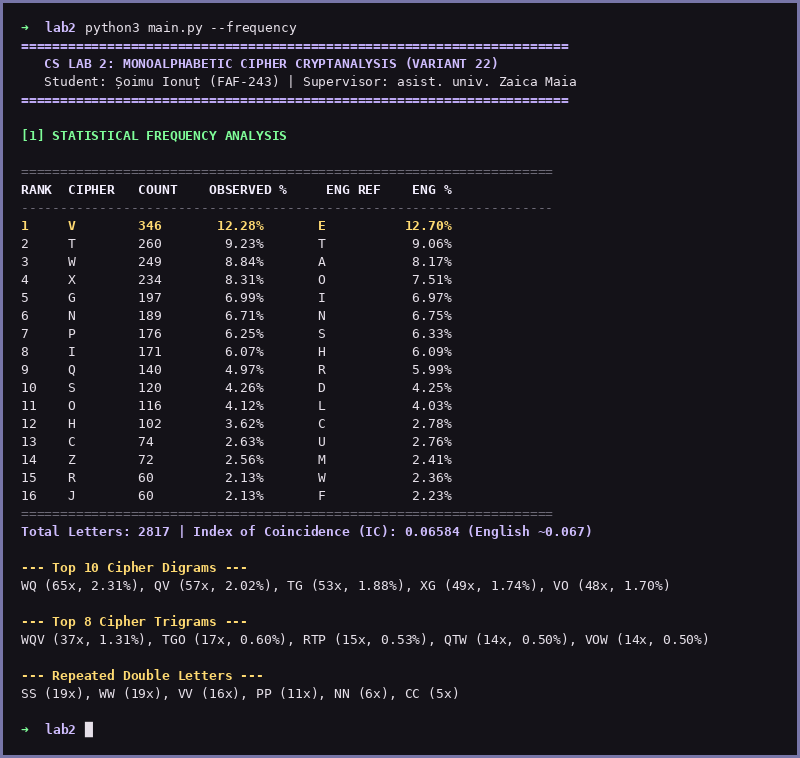
\includegraphics[width=0.88\linewidth]{figures/screenshot_frequency_analysis.png}
    \caption{Terminal capture: Statistical frequency analysis, N-gram distribution, and Index of Coincidence.}
    \label{fig:screen_freq}
\end{figure}

Figure~\ref{fig:screen_steps} illustrates the progressive deduction walkthrough generated by \texttt{python3 main.py --steps}, displaying the linguistic reasoning and partial decipherments from Milestone 1 through Milestone 4.

\begin{figure}[H]
    \centering
    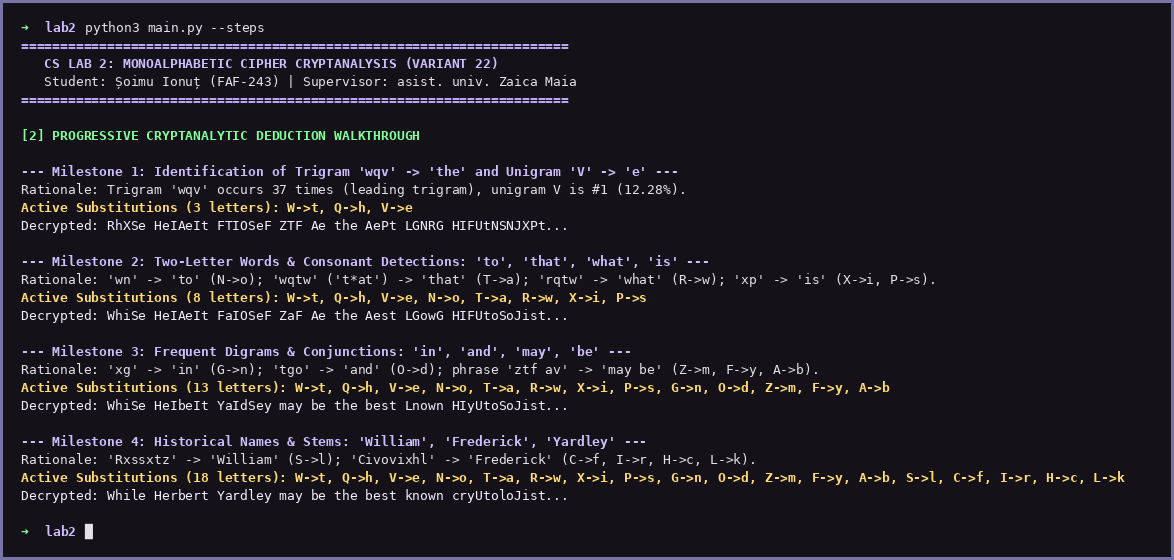
\includegraphics[width=0.88\linewidth]{figures/screenshot_step_decryption.png}
    \caption{Terminal capture: Step-by-step progressive cryptanalytic deduction walkthrough.}
    \label{fig:screen_steps}
\end{figure}

Figure~\ref{fig:screen_solve} demonstrates the full solution output generated by \texttt{python3 main.py --solve}, showing the reconstructed substitution key (Table 2.5), the affine algebraic parameters $E(x) = (7x + 19) \pmod{26}$, and the decrypted plaintext narrative.

\begin{figure}[H]
    \centering
    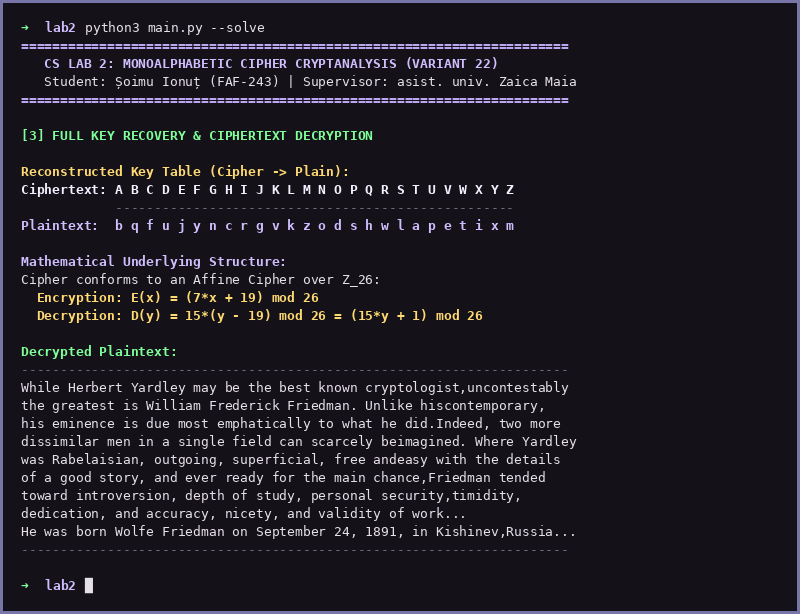
\includegraphics[width=0.88\linewidth]{figures/screenshot_final_decryption.png}
    \caption{Terminal capture: Recovered substitution alphabet table, affine formula, and decrypted plaintext.}
    \label{fig:screen_solve}
\end{figure}

\subsection{Full Decrypted Plaintext Narrative}

The complete decrypted text recovered from Variant 22 is presented below:

\begin{quote}
\small\itshape
While Herbert Yardley may be the best known cryptologist, uncontestably the greatest is William Frederick Friedman. Unlike his contemporary, his eminence is due most emphatically to what he did. Indeed, two more dissimilar men in a single field can scarcely be imagined. Where Yardley was Rabelaisian, outgoing, superficial, free and easy with the details of a good story, and ever ready for the main chance, Friedman tended toward introversion, depth of study, personal security, timidity, dedication, and accuracy, nicety, and validity of work. Despite the relative drabness of these personal traits—or perhaps because of them, Friedman's theoretical contributions and his practical attainments exceed those of any other cryptologist. Yardley's career was like an amazing skyrocket that explodes in fantastic patterns against the heavens. Friedman's was like the sun.

He was born Wolfe Friedman on September 24, 1891, in Kishinev, Russia, the oldest son and second child of Frederick and Rosa Friedman. His father, a Rumanian who spoke eight languages and worked as an interpreter for the Russian Post Office, emigrated to America in 1892, at which time his son's name was changed to William. The family settled in Pittsburgh, where his father managed a sewing machine agency. William graduated in 1909 as one of the ten honor students in a class of 300 at Pittsburgh Central High School; he then went to work as chief clerk in the Erie City Iron Works, a firm that sold steam engines. About that time the back-to-the-farm movement called to city boys, and in the fall of 1910, Friedman and three friends enrolled in Michigan Agricultural College, whose chief attraction was that it was tuition-free.

But Friedman soon discovered that farming held little interest for him. He was an inventive young fellow who liked to fix things and had written some science fiction for his high-school paper; he was rapidly coming to the conclusion that he liked science. At the end of the term he learned that tuition was also free in a scientific field allied to agriculture—genetics—at one of the Ivy League universities, Cornell. He borrowed train fare and arrived in Ithaca, New York, in February, 1911, where he got a job waiting on tables. After commencement in February of 1914, he attended graduate school, managing to fall in love twice, once with a brunette, once with the blonde daughter of a movie-house owner.

While he was there, a wealthy textile merchant, George Fabyan, who maintained laboratories in acoustics, chemistry, genetics, and cryptology (to try to prove that Bacon wrote Shakespeare's plays) on his 500-acre estate, Riverbank, at Geneva, Illinois, decided that he needed a geneticist to improve the grains and livestock on his farm. He applied to Cornell for a "would-be-er," not an "as-is-er," and hired Friedman, to begin June 1, 1915.

Fabyan was a man of no formal education but of intelligence and energy. He had a great desire to be "somebody," and that desire motivated his subsidizing the Baconian studies: proof of this revolutionary thesis would cover its patron as well as its actual discoverers with glory. He himself read little, but he absorbed enough from those around him to make his talk on almost any subject sound impressive—at least superficially. He was autocratic, never allowing his staff to disagree with him, but otherwise not unpleasant so long as employees recognized that he was boss. A cardinal article of faith with him was that a well-executed sales campaign could put across almost anything.
\end{quote}

% ==============================================================================
\section{Conclusions}
\markboth{7\quad Conclusions}{7\quad Conclusions}

In this laboratory work, I investigated and successfully implemented a cryptanalytic attack based on frequency analysis against a monoalphabetic substitution cipher (Variant 22).

\begin{itemize}[leftmargin=*]
    \item \textbf{Vulnerability of Monoalphabetic Systems:} Despite possessing an astronomically large theoretical key space ($26! \approx 4.03 \times 10^{26}$), monoalphabetic ciphers offer practically zero security against ciphertext-only attacks when messages exceed a few hundred characters. Because the substitution is stationary, all statistical properties of the natural language are preserved.
    \item \textbf{Statistical Indicators:} Computing the Index of Coincidence ($I_C = 0.06584$) accurately identified the underlying text as English monoalphabetic prose, ruling out polyalphabetic encryption and providing high confidence before undertaking manual deduction.
    \item \textbf{Synergy between Automation and Linguistic Deduction:} While pure mechanical frequency replacement often fails due to local statistical variations, pairing statistical sorting with progressive deduction (identifying short words like \texttt{the}, \texttt{to}, \texttt{is}, digram repetitions, and domain-specific terminology) enables efficient and unambiguous plaintext recovery.
    \item \textbf{Algebraic Cipher Structure:} Analysis of the recovered key revealed that the variant was systematically constructed using an Affine Cipher $E(x) = (7x + 19) \pmod{26}$, allowing mathematical confirmation of the linguistic decryption.
\end{itemize}

% ==============================================================================
\section{Source Code Repository}
\markboth{8\quad Source Code Repository}{8\quad Source Code Repository}

The complete Python implementation and report source files are hosted at:

\begin{center}
    \textbf{GitHub Repository Link:}\\
    \url{https://github.com/Lucariowu/cslabs/tree/main/lab2}
\end{center}

\end{document}
